\chapter{Auswertung und Vergleich mit Property-based Testing}
\label{experimente}

\section{Vergleichmetriken}
Bevor wir einen tatsächlichen Vergleich beider Methoden durchführen werden erst einmal die Metriken eingeführt, in denen sich Verglichen wird.
Hierdurch wird einfacher verständlich welche Punkte miteinander verglichen werden.
Wir nutzen die in \textit{Property-based Testing}~\cite{property-based-testing} genutzten Metriken.

\subsection{Metriken aus Property-based Testing}

In \textit{Property-based Testing} wurden zwei Metriken eingeführt, um die Methode zu evaluieren.
Hierbei wurden zwei Forschungsfragen entwickelt.

\begin{enumerate}
    \item Welche Schema Coverage kann mit der Methode erreicht werden?~\cite[vgl. RQ1]{property-based-testing}
    \item Wie gut ist die Fehlerfindungskapazität der Methode?~\cite[vgl. RQ2]{property-based-testing}
\end{enumerate}

Zur Beantwortung der Fragen wurden Experimente auf zwei Testsystemen ausgeführt.
Das erste Testsystem ist eine eigens entwickelte GraphQL-API die bekannte Fehler besitzt~\cite[vgl. A.1]{property-based-testing}.
Testsystem 2 ist GitLab.
Eine häufig genutzte Software für GitServer mit DevOps Kapazitäten.
Gitlab bietet seine API auch als GraphQL an und durch seine riesige Größe eignet sich GitLab als solides Testsystem.~\cite[vgl. A2]{property-based-testing}
Unser entwickelter Prototyp soll in exakt dem gleichen Umfeld seine Tests generieren.
Wir erwarten, dass wir möglichst dieselben Fehler finden wie die ursprüngliche Methode und ideal wäre es, wenn wir mehr und neue Fehler finden würden.
Beide Forschungsfragen werden im folgenden noch einmal näher erläutert da diese ein wenig spezialisiert sind und Wissen über Methode
ist wichtig um die Ergebnisse korrekt einordnen zu können.

\subsection{Fehlerfindungskapazitäten}

Mit Fehlerfindungskapazitäten ist gemeint wie zuverlässig die Methode tatsächliche Fehler findet.
Hierfür werden die beiden zuvor benannten APIs getestet und es wird geprüft, ob die Methode die Fehler finden konnte.
Um zu verifizieren, dass die Methode möglichst viele Fehler findet, gibt es eine Test API die
initial mit bekannten Fehlern versehen wird.
Die \textit{Property-based Methode} hat 11 von 15 Fehlern im speziell vorbereiteten System gefunden.
Bei GitLab wurden 4 Bugs im Query-Bereich gefunden.
Unsere entwickelte Methode soll mindestens die gleichen Fehler finden und idealerweise mehr.

\subsection{GraphQL-Schema Abdeckung}

Dadurch, dass \textit{Property-based Testing} auf zufallsbasierter Testgenerierung basiert stellt sich hier die Frage, wie gut die Methode
die API abdeckt und inwiefern die generierten Tests ausreichend sind.
Dies kommt insbesondere zu tragen, wenn die maximale Pfadlänge ausgehend vom Query Knoten größer ist als die erlaubte Rekursionstiefe des Prototypens.
In Property-based Testing wird definiert, dass die generierten Tests eine vollständige Abdeckung erreichen, wenn gilt:

\begin{definition}
    Für alle Objekte des Schemas: Bilde alle Tupel \{Object, Field \}.
    Ein Schema hat eine ideale Coverage, wenn alle Tupel durch einen Test abgedeckt sind. \cite[vgl. B. Measuring Schema Coverage ]{property-based-testing}
    \label{defedgecov}
\end{definition}

Es sei zuerst erwähnt, dass die hier angesprochene Abdeckung eine theoretische Abdeckung ist.
Die tatsächlich erreichte Abdeckung wird nicht betrachtet.

\section{Threats to Validity / Limitierungen}

Bevor wir mit dem eigentlichen Vergleich beginnen muss noch kurz eingeordnet werden, inwiefern die Experimente zu betrachten
sind und unter welchen Voraussetzungen der Vergleich geschieht.

\subsection{Argumentgeneratoren}

Wie in Kapitel~\ref{zufallsgen} erwähnt, ist es wichtig, dass GraphQL für jede Funktionen einen Wert ungleich $null$ bekommt, sodass der
Pfad weitergegangen werden kann und die Funktionen in diesem getestet werden um die tatsächliche Abdeckung zu erhöhen.
Um die Wahrscheinlichkeit zu erhöhen, dass Argumentgeneratoren ein Argument zurückliefern, dass zum SUT passt, wurden diese teilweise angepasst.
Wir verletzen hierbei nicht die Vergleichbarkeit der Arbeiten, da diese Anpassung der Argumengeneratoren in~\cite{property-based-testing} auch stattfand \cite[vgl. Experimental Setup and Method]{property-based-testing}.
Hierbei sei zum Beispiel erwähnt, dass eine Type $ID$ in GraphQL als String wert definiert ist, häufig in Implementierung jedoch als Zahlenstring genutzt wird.
Eine beispielhafte Anpassung wäre hier nun, dass wir den Generator für den Type $ID$ so anpassen, dass er nur Argumente für $ID$ zurückliefert die ein Zahlenwert sind
in einem gewissen Bereich der durch das SUT abgebildet wird.

\section{Fehlerfindungskapazitäten}

Zuerst wollen wir die Fehlerfindungskapazitäten des Prototypens beweisen.
Hierfür nutzen wir die beiden, zuvor benannten, Testsyteme GraphQL-Toy (eine experimentelle GraphQL-Implementierung) und GitLab in der Version 12.6.3.
Ziel ist es mindestens die Fehler zu finden die vom \textit{Property-based Testtool}\cite{property-based-testing} gefunden wurden.
Idealerweise wollen wir jedoch sogar mehr Fehler finden.

\subsection{GraphQL-Toy}

Das Testssystem GraphQL-Toy hat ein simples Schema in dem nur drei $OBJECT$ Typen exisitieren.
Diese sind $Query$, $Project$ und $User$.
Das Schema hat folgende Struktur: \\
\begin{center}
    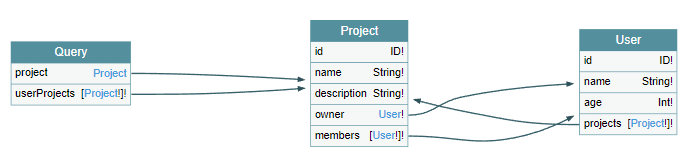
\includegraphics[width=\textwidth,height=\textheight,keepaspectratio]{img/graphqltoy}
\end{center}

Entwickelt wurde dieses System mit dem Hintergrund, dass bekannte Bugs im Code eingebracht werden und überprüft werden kann, ob das Testtool diese findet.
Insgesamt wurden 15 verschiedene Bugs eingefügt welche in verschiedene Kategorien fallen wie Syntaxfehler, falsche Rückgabedaten, falsche Datenstrukturen etc.
Einige der Bugs werden im folgenden kurz vorgestellt.
Eine Liste aller eingebauten Bugs lässt sich im Anhang unter \textit{GraphQL-Toy Implementation mit Bugs}~\ref{graphql-toy-code} finden.

\subsubsection{Bug 1 - SyntaxFehler}

Einfache Syntaxfehler wurden an verschiedenen Stellen eingebaut.
Dies bedeutet, dass jeder Funktionsaufruf dieser Funktion garantiert scheitern wird.
Somit kann jede Request diesen Fehlerfall entdecken, solange die Request auch das Feld hinter der Funktion mit dem Syntaxfehler abfragt.
Ein einfacher Syntaxfehler wäre zum Beispiel folgender Code: \\

\begin{lstlisting}[language=javascript]
    const resolvers = {
        Query: {
            project: (_, {id}, context, info) => {
                // Example bug 1 - Syntax mistake
                return db.projects.find(project => project.id ===);
            }
        }
    }
\end{lstlisting}

Hierbei fehlt der Wert mit dem die $project.id$ verglichen werden soll.
Ein jeder Aufruf dieser Funktion mit egal welcher $ID$ führt zu einem Fehler.

\subsubsection{Bug 2 - Falscher Objekttyp}

Objektfehler sind ein wenig unoffensichtlichere Fehler.
Hierbei gibt der Code ein Objekt zurück, dass nicht der definierten Struktur im Schema entspricht.
GraphQL wird hierfür dann einen Fehler erzeugen da die Daten eben nicht zum Schema passen.

\begin{lstlisting}[language=javascript]
    const resolvers = {
        Query: {
            project: (_, {id}, context, info) => {
                // Example bug 5 - wrong type "error"
                return { ...db.projects.find(project => project.id === id), name: ["a", "b"] };
            }
        }
    }
\end{lstlisting}

Um diesen Fehler ausführen zu können ist es wichtig, dass das Feld auch abgefragt wird.
Sollte das Feld ein Argument benötigen, so muss dieses passen, sodass auch wirklich ein Objekt abgefragt wird und dann der falsche Type zrückgegeben wird.

\subsubsection{Bug 3 - Typfehler in der Eingabe}

Felder wie $ID$ sind im GraphQL-Standard als einzigartige Strings definiert.
Im allgemeinen wird der $ID$ Type jedoch von diversen Entwicklern als Zahlenstring genutzt.
Eine Funktion wandelt diesen String dann in eine Zahl um die z.B. genutzt wird um einen bestimmten Eintrag eines Arrays zu bekommen.
Inputvalidierung ist also von Nöten.

\begin{lstlisting}[language=javascript]
    const resolvers = {
        Query: {
            project: (_, {id}, context, info) => {
                // Example bug 3 - Input type validation bug
                return db.projects[id];
            }
        }
    }
\end{lstlisting}

Es ist hier möglich, ohne jegliche Prüfung einen Key anzugeben.
Ist ein Resolver wie hier implementiert so ist es erlaubt in der Query jeglichen String anzugeben.
Es ist also sehr wahrscheinlich, dass beispielsweise ein IndexOutOfBound Fehler auftreten kann.
\\

Mit dem Testtool nach~\cite[Property-based Testing]{property-based-testing} konnten 73\% der Fehler, also 11 der 15 Fehler gefunden  werden.
Unser entwickeltes Testtool schaffte auf derselben API auch eine Entdeckung von 11 Fehlern.
Wir konnten also dieselbe Fehlerfindung erreichen wie das Property-based Tool.
Bemerkenswert hierbei ist allerdings, dass das Property-based Tool hierfür wesentlich mehr Queries benötigte, um eine zufriedenstellende Coverage zu erreichen.
Das Property-based Tool benötigte 30 Durchläufe, die jeweils bis zu 100\% Edge-Coverage liefen, um alle Fehler zu finden.
Im Kontrast dazu konnte unsere hier entwickelte Methode mithilfe von nur 2 PrimePfaden eine PrimePath Coverage erreichen.
Hierzu wurden für jeden Pfad 5 Testquerys entwickelt.
Es war somit möglich, alle 11 Fehler zu finden.
Bemerkenswert war, dass zwei perfekte Querys ermittelt wurden.
Das Testtool fand diese beiden Querys hierfür: \\

\begin{lstlisting}[language=GraphQL]
    { project(id: "2", ) {  id  name  description   owner {  id  name  age   }  }  }
\end{lstlisting}

\begin{lstlisting}[language=GraphQL]
    { userProjects(id: "1") { name owner { id name age projects { name description id } } } }
\end{lstlisting}

Mithilfe dieser Querys konnte jeder der 11 entdeckten Fehler gefunden werden.
Dies liegt auch daran, dass der Argumentgenerator entsprechend angepasst wurde und nur valide IDs produziert hat.
So war es sehr wahrscheinlich, dass eine ID die Generiert wird mindestens in einer der 5 erstellten Querys zur unterliegenden Datenstruktur gepasst hat
und wir somit die eine tatsächliche Testausführung haben und nicht nur einen initialen $null$ Wert der die Query sofort erfolgreich sein lässt.
Die 4 nicht gefundenen Fehler sind dieselben Fehler wie diese, die \textit{Property-based Testing}~\cite[vgl. RQ.2]{property-based-testing} nicht finden konnte.
Dies sind die Felder, in denen ein falscher Wert eines Objektes genutzt wurde, um ein anderes Objekt zu erlangen.
Hierbei verhindert der Black-Box Ansatz, dass der Fehler gefunden wird da eine leere Rückgabe des Feldes eine valide Antwort ist.
Wir wurden also limitiert vom Black-Box Ansatz, da das Verhalten für unseren Prototypen als fehlerfrei gilt es aber eigentliche eine fehlerhafte Ausgabe ist.
In diesem  Beispiel hat unser Prototyp die selben Fähigkeiten wie der Prototyp von \textit{Property-based Testing}.
Die Ergebnisse der Experimente befinden sich im \href{https://github.com/gernhard1337/GraphQL-Testautomatisierung/tree/main/experiment/toy-experiment}{GitHub}.

\subsection{GitLab}

Das Testsystem GitLab wurde schon in Property-based  Testing verwandt, um an einem Industry-ready Projekt die Methode zu evaluieren \cite[vgl. Experiment]{property-based-testing}.
Wir wollen unseren Prototypen auch an diesem System testen.
GitLab stellt sowohl eine REST als auch GraphQL-API zur Kommunikation  zur  Verfügung.
Mit GitLab wird ein komplexes Softwareprodukt zur Versionsverwaltung und DevOps-Anwendung getestet.
Die Komplexität dieser Software wird deutlich, wenn wir uns das GraphQL-Schema von GitLab ansehen welches in Abbildung~\ref{gitlabschema} gezeigt wird.
Eine hochauflösendere Version ist im \href{https://github.com/gernhard1337/GraphQL-Testautomatisierung/blob/main/latex/img/gitlabgraph.png}{GitHub} verfügbar.
Das Schema ist sehr komplex und stark zyklisch.

\begin{figure}[H]
    \begin{center}
        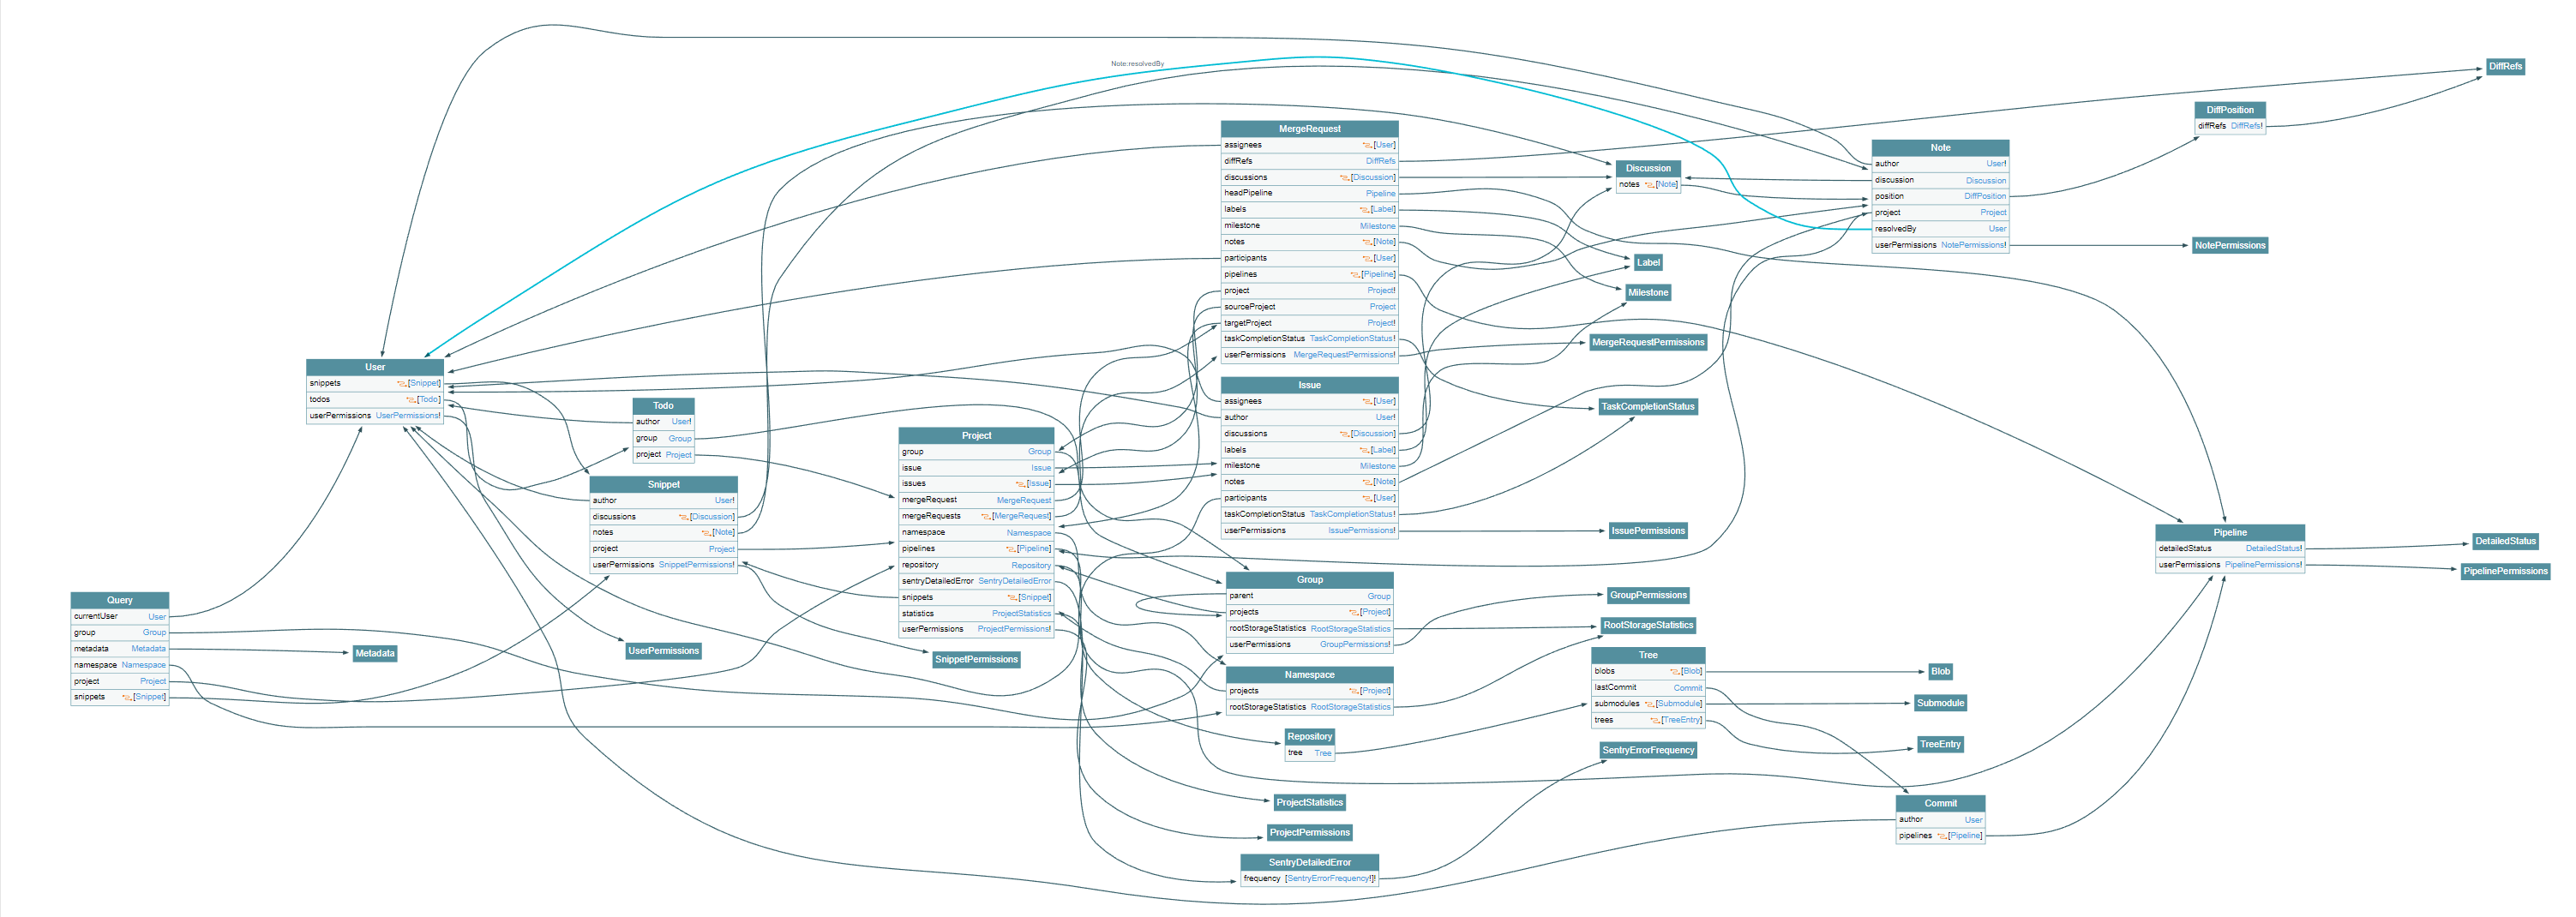
\includegraphics[width=\textwidth,height=\textheight,keepaspectratio]{img/gitlabgraph}
    \end{center}
    \caption{GitLab GraphQL-Schema}
    \label{gitlabschema}
\end{figure}

Das \textit{Property-based Testtool} fand insgesamt 4 Fehler die im Query-Bereich von GraphQL waren.
Alle Fehler waren Fehler in der Validierung von Eingabevariablen.
Hierbei lag der Fehler darin, dass die Resolver einen Fehler verursachten, wenn als Eingabe ein String mit leerem Zeichen kam.
Dies bedeutet, ein leerer String \verb+""+ wird richtig behandelt (außer ein Fehler 4) aber ein String mit leerem Zeichen führt zum Fehler: \verb+e\u0000\+
Die Fehler wurden gefunden durch folgende Querys:

\begin{lstlisting}[language=GraphQL, caption=Fehler 1\cite{issue1}]
{project(fullPath: "root/test-project") {sentryDetailedError(id: "") {count}}}
\end{lstlisting}

\begin{lstlisting}[language=GraphQL, caption=Fehler 2\cite{issue2}]
{project(fullPath: "e\u0000") {name fullPath}}
\end{lstlisting}

\begin{lstlisting}[language=GraphQL, caption=Fehler 3\cite{issue3}]
{namespace(fullPath: "e\u0000") {fullName name fullPath}}
\end{lstlisting}

\begin{lstlisting}[language=GraphQL, caption=Fehler 4\cite{issue4}]
{group(fullPath: "e\u0000"){fullName name fullPath }}
\end{lstlisting}

Alle vom Property-based Tool gefunden Fehler wurden durch unseren Prototypen gefunden mit den Querys

\hyperref[query1]{Query 1},
\hyperref[query2]{Query 2},
\hyperref[query3]{Query 3} und
\hyperref[query4]{Query 4}.

Getestet wurde auf dem offiziellen GitLab-Docker Image in der Version 12.6.3
Damit im GitLab auch Daten verfügbar sind wurde ein Population-Skript geschrieben, dass im GitLab
50 User anlegt und jedem User einige Projekte, Commit, MergeRequests usw. zuordnet.
Das Population-Skript kann im~\cite[Github]{populationscript} gefunden werden.
Da die Querygenerierung stets im Query-Knoten beginnt und die PrimePaths gefunden werden sollen, ergeben sich in diesem Schema sehr viele ähnliche Querys.
Diese unterscheiden sich insbesondere am Ende der jeweiligen Query.
Der zuvor vorgestellte Algorithmus errechnet für das Schema von GitLab eine Pfadanzahl von 41744 für eine PrimePath-Coverage des Schemas.
Eine genaue Auflistung aller Pfade findet sich im~\cite[GitHub]{gitlabpaths}.
Mit der Maßgabe, dass wir pro Pfad 5 Tests erzeugen wollen wurden dann 208.720 Tests erzeugt.
In nahezu allen Fällen haben die generierten Tests eine tatsächliche Pfadlänge die kleiner ist als die erwartete.
Dies begründet sich daran, dass an verschiedenen Stellen des Schemas von GitLab Argumente angegeben werden müssen
und mit jedem Argument das zusätzlich generiert wird, steigt die Wahrscheinlichkeit, dass die zufällige Kombination unpassend ist.
In mehreren Durchläufen zeigte sich, dass im Schnitt nur ungefähr 20 Tests eine ideale Pfadlänge erreichen.
Die Tests, die das erreichen sind im allgemeinen auch Tests, die einen sehr kurzen Pfad abbilden.
Hier verringert sich einfach das Risiko, dass Eingabeargumente generiert werden, die keine zugrundeliegenden Daten haben und somit die Pfadausführung verhindern.
Ein Beispiel hierfür ist der Pfad $Query -> Project -> MergeRequest -> Time$

\begin{lstlisting}[language=GraphQL]
{ project(fullPath: "groupx_3/projectx_2_1") {
    archived
    avatarUrl
    containerRegistryEnabled
    ...
    mergeRequest(iid: "1") {
        allowCollaboration
        createdAt
        mergeStatus
        ...
        }
    }
}
\end{lstlisting}

durch gutes Mocken des FullPath Argumentgenerators war es möglich, eine Query zu generieren, die somit passende Argumente generiert hat um für eine ideale Testausführung (d.h. Länge Ergebniss = Länge Testpfad) zu sorgen.
Generell zeigt sich sehr schnell, dass bei unserer Methode ähnliche Limitierungen wie im Property-based Testing auftreten.
So ist eine Anpassung an das Domänenwissen nötig.
Für GitLab bedeutet dies unter anderem, dass die ID-Struktur um zum Beispiel Projekte abzufragen in der Form \verb+<user>/<project>+ sein muss.~\cite[vgl. S.8]{property-based-testing}
Da wir ähnliche Argumentgeneratoren verwendet haben wie in Property-based Testing, haben wir auch deren Limitierungen von mangelndem Domänenwissen~\cite[vgl. S.8]{property-based-testing}.
Wir generieren zwar sehr viele Tests die PrimePfad Abdeckung umsetzen.
Wenn jedoch die Generierung der Tests auf Zufall basiert, so können wir auch nicht garantieren, dass unsere Eingabeargumente passend sind und ein valides Ergebniss zurückgeben.
Wird kein Ergebniss zurückgegeben, so folgert GraphQL, dass spätere Funktionen nicht ausgeführt werden müssen und somit werden diese auch nicht getestet.
Es ist möglich, dieses Problem zu beheben, hierzu jedoch in Kapitel~\ref{futurework} mehr.

\section{Schema-Abdeckung}

Wie in Property-based Testing schon erwähnt: \textit{da keine Coverage Metric für GraphQL Blackbox Test Auswertung exisitiert, starten wir mit einem sehr
einfachen und intuitiven Ansatz}~\cite[vgl. B. Measuring Schema Coverage]{property-based-testing}.
In der Tat ist das vorgestellte Abdeckungskriterium ein sehr einfaches Kriterium.
Es lässt zum Beispiel die Beziehungen zwischen allen Knoten aus und beachtet nur, dass alle Knoten inbegriffen sind mit allen Feldern.
Hiermit entspricht das definierte Abdeckungskriterium der Kantenabdeckung nach Definition~\ref{kantenabdeck}.
Denn alle Knoten müssen abgedeckt sein und alle Kanten ausgehend von den Knoten.
Da jedoch das Rekursionslimit die Pfadlänge begrenzt, wird der Graph des Schemas künstlich beschnitten und alle Pfade die länger als
das Rekursionslimit sind, werden in der Abdeckung nicht berücksichtigt.
Hierdurch folgt, dass sich die gewünschte Kantenabdeckung in Realität nicht zuverlässig ergibt, da GraphQL-Schemas durchaus Pfadlängen länger
als das Rekursionslimit zulassen (das Rekursionslimit wurde standardmäßig auf 4 gesetzt \cite[vgl. SourceCode ]{property-based-testing}).
Um die gewünschte Kantenabdeckung zu erreichen musste im \textit{Property-based Testing} außerdem die Generierung mehrfach ausgeführt werden
bis die Abdeckung erreicht wurde.
Um eine vollständige Abdeckung beim GitLab Schema zu erreichen waren diverse Iterationen nötig bei verschiedenen Rekursionslimits.
Eine 100\% Coverage wurde bei GitLab nur in einem Versuch erreicht, wenn 10000 Tests mit Rekursionslimit 4 erstellt wurden \cite[vgl. Tabelle 2]{property-based-testing}.
Da der Graph des GitLab-Schemas jedoch beschnitten wurde, da dieser wie wir später sehen werden wesentlich größer ist, kann nicht gesagt werden,
dass vollständige Kantenabdeckung erreicht wurde.
Der wesentliche Unterschied beider Methoden ist, dass \textit{Property-based Testing} Experimente für die theoretische Abdeckung ausführen muss
und hierbei mehrere Iterationen benötigt um diese zu erreichen.
Der Ansatz der PrimePfad-Abdeckung in unserem Prototypen stellt sicher, dass die generierten Pfade PrimePfade sind.
Wir stellen somit sicher, dass stets die Abdeckung erfüllt ist.
Gleichzeitig nutzen wir ein stärkeres Abdeckungskriterium auf unbeschnittenen Graphen.
Man kann also folgern, dass unsere Methode eine starke Verbesserung der theoretischen Abdeckung erzielt hat.
Die Limitierung der zufälligen Argumentgeneratoren behindern eine tatsächliche Umsetzung der theoretischen Abdeckung.
Allerdings ist diese Limitierung potentiell lösbar, hierzu in Kapitel~\ref{futurework} mehr.
\newpage

\subsection{GraphQL-Toy Schema Coverage}

Wie eingeführt in \textit{Property-based Testing}~\cite{property-based-testing} muss für eine zufriedenstellende Abdeckung
die Defintion~\ref{defedgecov} erfüllt sein, dass jedes Paar von \verb+(Type, objectField)+ berücksichtigt ist.
Dies bedeutet für das Schema, dass die folgenden Tupel abgedeckt sein müssen um Kantenabdeckung zu erfüllen.
    \begin{itemize}
        \item \verb+(Query, project)+
        \item \verb+(Query, userProject)+
        \item \verb+(Project, owner)+
        \item \verb+(Project, members)+
        \item \verb+(User, projects)+
    \end{itemize}

Da nur die beiden initialen Felder aus dem Query-Type Eingabeargumente benötigen ist die Querygenerierung simpel.
Wir können keine Aussage darüber machen, ob die generierten Querys von \textit{Property-based Testing}\cite{property-based-testing} diese Coverage erfüllen denn bei der Querygenerierung spielt es keine Rolle ob dieses Measurement erreicht wird.
Es gibt lediglich eine Messung die zeigt, dass der Prototyp mit hinreichender Wahrscheinlichkeit in der Lage ist, durch zufällige Querygenerierung Tests zu generieren, die Edge-Coverage erfüllen. \cite[vgl. D.Results RQ1 ]{property-based-testing}.
Im Gegensatz zum Property-based Testing hat der hier entwickelte Prototyp den Vorteil, dass die Pfadgenerierung nicht zufällig ist.
Wir berechnen PrimePfade, diese sind in einem stärkeren Abdeckungskriterium enthalten als die Kantenabdeckung.
Dadurch ergibt sich, dass die Tests, die vom hier entwickelten Prototyp erstellt werden, stets auch die Kantenabdeckung erfüllen.
Die Abdeckung muss nun also nicht mehr durch hinreichend viele Tests sichergestellt werden.
Ein einziger Durchlauf reicht aus, um sicherzustellen, dass die gewünschte Coverage erreicht ist.
Natürlich bleibt offen, ob die generierten Tests diese Coverage tatsächlich erreichen jedoch ist dies auch ein Problem im Property-based Testing.
Dort wird auch nur geprüft, ob die Felder in der Anfrage existieren jedoch nicht, ob die Antwort diese auch enthält.
Um dies messbar zu machen haben wir zuvor die Pfadlängen eingeführt.
Hierdurch konnten wir zeigen, dass die generierten Querys in Teilen die Abdeckung auch tatsächlich umsetzen.

\subsection{GitLab Schema Coverage}

Das GitLab Schema ist wesentlich komplexer.
Im Gegensatz zum GraphQL-Toy besteht das GitLab Schema aus 37 Knoten welche jeweils zahlreiche Kanten hinzufügen.
Generell lässt sich sagen, dass das Schema sehr komplex und stark rekursiv ist.~\cite[vgl. Studied Cases 2]{property-based-testing}
Da der Property-based Testing Ansatz ein Rekursionslimit benötigt stellt, sich hier die Frage inwiefern überhaupt das Schema überdeckt werden kann.
Laut Paper hat sich ein Rekursionslimit von 4 als hinreichend ausgezeichnet~\cite[vgl. Table 1 ]{property-based-testing} und wurde auch so im Code übernommen.
Ein Rekusionslimit von 4 bedeutet, dass die maximale zu erreichende Pfadlänge des Testpfades 4 ist.
Da das GitLab-Schema aber nun einen Graphen aufspannt, der durchaus wesentlich längere Pfade als 4 hat, ist es fragwürdig wie die 100\% Schema-Coverage in~\cite[Table 1]{property-based-testing} berechnet wurden.
Es seien hier einige Pfade beispielhaft genannt, die einzigartig sind, bei denen sich keine Kante doppelt und deren Länge 4 stark überschreitet: \\

\begin{itemize}
    \item Query \textrightarrow User \textrightarrow SnippetConnection \textrightarrow SnippetEdge \textrightarrow Snippet \textrightarrow DiscussionConnection \textrightarrow DiscussionEdge \textrightarrow Discussion \textrightarrow NoteConnection \textrightarrow NoteEdge \textrightarrow Note \textrightarrow Project \textrightarrow IssueConnection \textrightarrow Issue \textrightarrow Milestone \textrightarrow Time
    \item Query \textrightarrow Project \textrightarrow Issue \textrightarrow DiscussionConnection \textrightarrow DiscussionEdge \textrightarrow Discussion \textrightarrow NoteConnection \textrightarrow NoteEdge \textrightarrow Note \textrightarrow User \textrightarrow SnippetConnection \textrightarrow SnippetEdge \textrightarrow Snippet \textrightarrow Time \\
    \item Query \textrightarrow Namespace \textrightarrow ProjectConnection \textrightarrow Project \textrightarrow MergeRequestConnection \textrightarrow MergeRequestEdge \textrightarrow MergeRequest \textrightarrow UserConnection \textrightarrow User \textrightarrow SnippetConnection \textrightarrow Snippet \textrightarrow DiscussionConnection \textrightarrow PageInfo \\
\end{itemize}

Durch die Beschneidung des Graphens in \textit{Property-based Testing} durch das Rekursionslimit folgt, dass die ermittelte Kantenabdeckung
nicht zutreffend ist und nur für einen Teilgraphen des gesamten Graphens zutrifft.
Dies ist ein sehr großer, struktureller Einschnitt und die in Property-based Testing genannten 100\% Kantenabdeckung ist keine tatsächliche Kantenabdeckung,
sondern eben nur für den abgeschnittenen Teilgraphen.
Wie auch zuvor erwähnt, erzeugt unser hier entwickelter Prototyp Tests, die PrimePfad-Abdeckung umsetzen und somit ein stärkeres Abdeckungskriterium ist.
Wir führen die Pfadgenerierung auf dem gesamten Graphen aus und erhalten, wie zuvor erwähnt, über 40.000 Pfade zurück die nötig sind um eine PrimePath-Coverage für das GitLab Schema zu erreichen.
Hier zeigt sich auch ein direkter Unterschied.
Während in Property-based Testing gesagt wird, dass 10.000 Tests mit einem Rekursionslimit von 4 ausreichen um ein 100\% Edge-Coverage zu erreichen~\cite[vgl. Table 1]{property-based-testing}
so sehen wir, dass 10.000 Tests nicht reichen können, wenn über 40.000 PrimePaths existieren.
Insbesondere sei hierbei angemerkt, dass die Pfad- \& Testgenerierung auf dem GitLab-Schema keine allzu rechenintensive Aufgabe war.
Die Berechnung der Querys geschah auf einem hardwaretechnisch ähnlichem Level wie in Property-based Testing verwandt.~\cite[vgl. Experimental Setup]{property-based-testing}.
Hier wurde die Aussage getroffen, dass ein~\cite[Tiefensuchen Ansatz nicht skaliert und deswegen ein iterativer Ansatz zu präferieren ist]{property-based-testing}.
Der hier entwickelte Prototyp zeigt das Gegenteil.

\section{Zusammenfassung der Experimente}

Wir konnten in beiden Experimenten zeigen, dass unser Prototyp dieselben Fehler findet wie der Prototyp aus Property-based Testing.
Es wurde gezeigt, dass die theoretische Abdeckung eines GraphQL-Schemas mit unserem Prototypen immens gesteigert wird ohne,
wie in~\cite{property-based-testing} behauptet, die Berechnungszeit signifikant zu erhöhen.
Während wir die theoretische Abdeckung des Graphens erhöhen konnten, so zeigte sich, dass die reale Abdeckung nicht mit der
theoretischen Abdeckung mithalten kann.
Die Pfadlänge der generierten PrimePfade ist im Allgemeinen sehr lang und hierdurch steigt die Wahrscheinlichkeit, dass ein Pfad eben nicht komplett ausgeführt wird.
Eine Anpassung der Argumentgeneratoren an das jeweilige SUT ist sinnvoll und verbessert die Pfadlängen der Tests.
Unser Prototyp leidet unter der selben Limitierung wie das \textit{Property-based Testing} indem wir mehr Domänenwissen über die
zugrundeliegenden Resolver und Daten haben müssen um sinnvolle Test zu generieren.
Dies ist Analog zu~\cite{property-based-testing} wo es heißt: \textit{.. das Domänenwissen von zugrundeliegenden Entitäten eine stärkere Testumgebung erzeugen kann}~\cite[S.8]{property-based-testing}
Möglichkeiten um das Domänenwissen über das SUT zu erhöhen ergründen wir in Kapitel~\ref{futurework}